% Options for packages loaded elsewhere
\PassOptionsToPackage{unicode}{hyperref}
\PassOptionsToPackage{hyphens}{url}
\PassOptionsToPackage{dvipsnames,svgnames,x11names}{xcolor}
%
\documentclass[
  10pt,
  letterpaper,
  DIV=11,
  numbers=noendperiod]{scrartcl}

\usepackage{amsmath,amssymb}
\usepackage{iftex}
\ifPDFTeX
  \usepackage[T1]{fontenc}
  \usepackage[utf8]{inputenc}
  \usepackage{textcomp} % provide euro and other symbols
\else % if luatex or xetex
  \usepackage{unicode-math}
  \defaultfontfeatures{Scale=MatchLowercase}
  \defaultfontfeatures[\rmfamily]{Ligatures=TeX,Scale=1}
\fi
\usepackage{lmodern}
\ifPDFTeX\else  
    % xetex/luatex font selection
\fi
% Use upquote if available, for straight quotes in verbatim environments
\IfFileExists{upquote.sty}{\usepackage{upquote}}{}
\IfFileExists{microtype.sty}{% use microtype if available
  \usepackage[]{microtype}
  \UseMicrotypeSet[protrusion]{basicmath} % disable protrusion for tt fonts
}{}
\makeatletter
\@ifundefined{KOMAClassName}{% if non-KOMA class
  \IfFileExists{parskip.sty}{%
    \usepackage{parskip}
  }{% else
    \setlength{\parindent}{0pt}
    \setlength{\parskip}{6pt plus 2pt minus 1pt}}
}{% if KOMA class
  \KOMAoptions{parskip=half}}
\makeatother
\usepackage{xcolor}
\setlength{\emergencystretch}{3em} % prevent overfull lines
\setcounter{secnumdepth}{-\maxdimen} % remove section numbering
% Make \paragraph and \subparagraph free-standing
\ifx\paragraph\undefined\else
  \let\oldparagraph\paragraph
  \renewcommand{\paragraph}[1]{\oldparagraph{#1}\mbox{}}
\fi
\ifx\subparagraph\undefined\else
  \let\oldsubparagraph\subparagraph
  \renewcommand{\subparagraph}[1]{\oldsubparagraph{#1}\mbox{}}
\fi


\providecommand{\tightlist}{%
  \setlength{\itemsep}{0pt}\setlength{\parskip}{0pt}}\usepackage{longtable,booktabs,array}
\usepackage{calc} % for calculating minipage widths
% Correct order of tables after \paragraph or \subparagraph
\usepackage{etoolbox}
\makeatletter
\patchcmd\longtable{\par}{\if@noskipsec\mbox{}\fi\par}{}{}
\makeatother
% Allow footnotes in longtable head/foot
\IfFileExists{footnotehyper.sty}{\usepackage{footnotehyper}}{\usepackage{footnote}}
\makesavenoteenv{longtable}
\usepackage{graphicx}
\makeatletter
\def\maxwidth{\ifdim\Gin@nat@width>\linewidth\linewidth\else\Gin@nat@width\fi}
\def\maxheight{\ifdim\Gin@nat@height>\textheight\textheight\else\Gin@nat@height\fi}
\makeatother
% Scale images if necessary, so that they will not overflow the page
% margins by default, and it is still possible to overwrite the defaults
% using explicit options in \includegraphics[width, height, ...]{}
\setkeys{Gin}{width=\maxwidth,height=\maxheight,keepaspectratio}
% Set default figure placement to htbp
\makeatletter
\def\fps@figure{htbp}
\makeatother

\usepackage{float}
\usepackage{tabularray}
\usepackage[normalem]{ulem}
\usepackage{graphicx}
\UseTblrLibrary{booktabs}
\UseTblrLibrary{rotating}
\UseTblrLibrary{siunitx}
\NewTableCommand{\tinytableDefineColor}[3]{\definecolor{#1}{#2}{#3}}
\newcommand{\tinytableTabularrayUnderline}[1]{\underline{#1}}
\newcommand{\tinytableTabularrayStrikeout}[1]{\sout{#1}}
\KOMAoption{captions}{tableheading}
\usepackage{float}
\floatplacement{table}{H}
\makeatletter
\@ifpackageloaded{caption}{}{\usepackage{caption}}
\AtBeginDocument{%
\ifdefined\contentsname
  \renewcommand*\contentsname{Table of contents}
\else
  \newcommand\contentsname{Table of contents}
\fi
\ifdefined\listfigurename
  \renewcommand*\listfigurename{List of Figures}
\else
  \newcommand\listfigurename{List of Figures}
\fi
\ifdefined\listtablename
  \renewcommand*\listtablename{List of Tables}
\else
  \newcommand\listtablename{List of Tables}
\fi
\ifdefined\figurename
  \renewcommand*\figurename{Figure}
\else
  \newcommand\figurename{Figure}
\fi
\ifdefined\tablename
  \renewcommand*\tablename{Table}
\else
  \newcommand\tablename{Table}
\fi
}
\@ifpackageloaded{float}{}{\usepackage{float}}
\floatstyle{ruled}
\@ifundefined{c@chapter}{\newfloat{codelisting}{h}{lop}}{\newfloat{codelisting}{h}{lop}[chapter]}
\floatname{codelisting}{Listing}
\newcommand*\listoflistings{\listof{codelisting}{List of Listings}}
\makeatother
\makeatletter
\makeatother
\makeatletter
\@ifpackageloaded{caption}{}{\usepackage{caption}}
\@ifpackageloaded{subcaption}{}{\usepackage{subcaption}}
\makeatother
\ifLuaTeX
  \usepackage{selnolig}  % disable illegal ligatures
\fi
\usepackage{bookmark}

\IfFileExists{xurl.sty}{\usepackage{xurl}}{} % add URL line breaks if available
\urlstyle{same} % disable monospaced font for URLs
\hypersetup{
  pdftitle={Understanding the Impact of Socioeconomic and Regional Factors on Health and Educational Outcomes},
  pdfauthor={Rishika Randev, Jenny Wu, Uzoma Uwazurike Jr., Shiyue Zhou},
  colorlinks=true,
  linkcolor={blue},
  filecolor={Maroon},
  citecolor={Blue},
  urlcolor={Blue},
  pdfcreator={LaTeX via pandoc}}

\title{Understanding the Impact of Socioeconomic and Regional Factors on
Health and Educational Outcomes}
\author{Rishika Randev, Jenny Wu, Uzoma Uwazurike Jr., Shiyue Zhou}
\date{}

\begin{document}
\maketitle

\subsection{Abstract}\label{abstract}

This study examines the relationships between socioeconomic, health, and
educational indicators in U.S. counties using data from the County
Health Rankings \& Roadmaps program and IPUMS. We analyze how factors
such as residential segregation, health insurance coverage, access to
healthy foods, and region impact life expectancy, and how residential
segregation and region affect school funding adequacy. Our findings
reveal that life expectancy is influenced by residential segregation and
uninsured rates, though these effects are minor compared to the more
substantial influence of household income and regional differences. Life
expectancy averages are highest in the Northeast, followed by the
Midwest, West, and South. Region also plays the most significant role
out of all included variables in determining the likelihood of school
funding adequacy, with schools in the Northeast and Midwest being far
more likely to receive adequate funding than those in the South. Other
factors, such as residential segregation, property taxes, and household
income, show statistically significant but smaller effects. These
results highlight the complex interplay between socioeconomic variables
and geographic location in shaping public well-being. By identifying key
disparities in health and education, this study underscores the
importance of equitable resource allocation and targeted policies to
address regional and socioeconomic inequalities.

\subsection{\texorpdfstring{\textbf{Introduction}}{Introduction}}\label{introduction}

Life expectancy and school funding are important indicators of public
well-being because they capture fundamental aspects of health,
education, and social equity that are essential for the development of
individuals and communities. Life expectancy is an important indicator
that reflects not only the overall health of a society, but also its
stability, economic resilience, and levels of inequality. While access
to quality healthcare and nutritious foods are drivers of well-being,
where you live and the nature of the community you live in likely also
have an influence on health outcomes such as life expectancy. According
to ``The Root Causes of Health Inequity - Communities in Action'' report
from the National Institutes of Health, we can infer that differences in
life expectancy between regions and socioeconomic groups often reveal
systemic inequalities, with marginalized communities experiencing
shorter life spans due to limited access to health care, healthy living
environments, and economic opportunities.\textsuperscript{1}~When it
comes to educational indicators, adequately funded schools ensure that
students have equal access to learning opportunities, serving as a
crucial investment in social mobility. The Stanford Center for
Opportunity Policy in Education highlights that ``the unequal allocation
and inadequate levels of resources in schools and communities {[}are{]}
at the heart of many gaps in student opportunity.''\textsuperscript{2}
This emphasizes the importance of equitable and adequate school funding
in closing opportunity gaps and empowering students from disadvantaged
backgrounds to achieve academic and economic success. By better
understanding the correlates of school funding adequacy, we can take a
major step towards implementing policy that targets the areas and
communities most affected by this issue.

For this purpose, we focus our analysis on two key research questions.
First, we investigate how socioeconomic factors impact average life
expectancy. \textbf{We seek to answer the question, ``What is the impact
of residential segregation, access to healthy foods, and health
insurance coverage on a county's average life expectancy?''.} This
analysis includes a comparison across different regions to identify
variations in the relationship between residential segregation and life
expectancy. Second, \textbf{we seek to answer the question, ``Do
residential segregation and region impact the likelihood of a school
being adequately funded?''}. This question allows us to assess how the
racial makeup and geographic location---given that each region of the
U.S. is characterized by differing political and cultural norms---affect
a county's educational investment. The observational unit for this
analysis is the U.S. county.

To obtain data on the aforementioned variables, we used three primary
sources.~

The first source was the County Health Rankings \& Roadmaps
program,\textsuperscript{3} associated with the University of Wisconsin
Population Health Institute, which provided us with 2024 datasets for
all U.S. states. This program consolidates the latest county-level
measurements of various population health, economic, demographic, and
social factors from the American Community Survey, the USDA Food
Environment Atlas, Small Area Income and Poverty Estimates, and other
reliable government sources into publicly available datasets every year.
Our specific variables of interest were originally collected as part of:

\begin{itemize}
\item
  National Center for Health Statistics - Natality \& Mortality Files,
  2019-2021 (average life expectancy)
\item
  American Community Survey 5-year estimates, 2018-2022 (residential
  segregation index \& median household income)
\item
  USDA Food Environment Atlas, 2019 (percentage of population with
  limited access to healthy foods)
\item
  Small Area Health Insurance Estimates, 2021 (percentage of adults
  uninsured)
\item
  School Finance Indicators Database, 2021 (school funding adequacy)
\end{itemize}

The second source was IPUMS, which provided us with median poverty tax
data for every county from 2018-2022.\textsuperscript{4}

The third source was the U.S. Census Bureau's Regions and Divisions of
the United States, which maps every U.S. to one of four geographic
regions, and also a division within the regions. We specifically
included regions as a variable in this analysis.~This data was loaded
into R using a
\href{https://github.com/cphalpert/census-regions}{publicly available
GitHub repository} titled \emph{Census Regions}.\textsuperscript{5}

\subsection{\texorpdfstring{\textbf{Methods}}{Methods}}\label{methods}

\subsubsection{Variable Selection}\label{variable-selection}

Variables of interest were selected \emph{a priori} based on their
perceived relevance to the two outcomes we wanted to better understand:
average life expectancy and school funding adequacy. While nutrition and
access to quality healthcare are inherently linked to general wellbeing,
it is worthwhile to assess how influential the environmental and
financial aspects of these factors are on our tangible outcome.
Therefore, we selected two key predictors for our life expectancy model:
the percentage of the population with limited access to healthy foods
and the percentage of uninsured adults in a county. The former is
defined by the US Department of Agriculture as ``the percentage of the
{[}county{]} population that is low-income and does not live close to a
grocery store'', where ``close'' is defined differently for rural and
nonrural areas.\textsuperscript{6} The latter variable represents the
percentage of adults in a county younger than 65 who lack health
insurance. We also were interested in seeing how residential segregation
would impact life expectancy among these predictors, given existing
studies on the negative health effects of segregation, and whether this
relationship would exhibit any variations across different regions. This
is why we chose to include residential segregation index values as a
predictor. The residential segregation index, used by the County Health
Rankings \& Roadmaps program, measures how evenly two groups, such as
Black and white residents, are distributed across geographic areas, with
values ranging from 0 (complete integration) to 100 (complete
segregation).\textsuperscript{7}~

Past studies have established a correlation between income and life
expectancy.\textsuperscript{8} Because we wanted to control for its
effects and examine how insurance, healthy food access, segregation, and
region influence life expectancy even within a given income bracket, we
selected income as our final predictor for the first model.

School funding adequacy is defined by the County Health Rankings program
as ``the average dollar gap between actual per-pupil spending and the
amount needed for students to achieve national average test scores,
considering districts' varying equity-based needs.''\textsuperscript{9}
To explore how racial diversity interface with variations in school
funding, we selected residential segregation to be a part of this
regression. In addition, given that state policy has a large influence
on school administration and the determination of school needs, and that
states in the same region tend to have similar political leanings and
cultural beliefs, we wanted to analyze how much of a relationship exists
between region and actual school funding levels. Because a major source
of public school funding is tax revenue, median property tax and median
household income were also included in the school funding model as
potential confounders. This allowed us to assess whether the effects of
segregation and region on funding existed outside of the effects of
known economic factors.

\subsubsection{Exploratory Data Analysis \& Data
Preprocessing}\label{exploratory-data-analysis-data-preprocessing}

2024 datasets for all U.S. states were combined and merged with median
property tax and region mapping data, resulting in a final dataset with
3144 county observations and 9 different variables (state, average life
expectancy, residential segregation index, \% limited access to healthy
foods, \% uninsured adults, school funding adequacy, median household
income, median property tax, and region). Because school funding
adequacy was given as a numerical value, and we wanted to focus on
better understanding the dichotomy between school funding adequacy and
inadequacy, this variable was converted into a binary categorical
variable (where the value was set to 1 if the numerical value was
positive, indicating the counties' schools were adequately funded, and
set to 0 if the numerical value was negative, indicating underfunding).

Exploratory data analysis for the two outcome variables was conducted by
1) calculating descriptive statistics, 2) creating scatterplots of each
individual predictor against the outcome (for life expectancy), and 3)
creating pairwise plots between variables (for school funding). During
the initial stages of analysis, we found that ⅓ of our observations were
missing residential segregation index data, and that certain states were
missing nearly all of their segregation values. Because of this, we
decided to drop all states missing over 50\% of their values for any
variable. This led to our analysis being limited to 33 states, and
excluding the following: Alaska, Colorado, Idaho, Iowa, Kansas,
Minnesota, Montana, Nebraska, North Dakota, South Dakota, Utah, Wyoming,
and Vermont. We were left with 2379 total observations, and the missing
percentage for residential segregation dropped to 22\%.

After this, the remaining missing values in all variables were imputed
using the mice package and predictive mean matching to generate one
complete dataset. The original school funding adequacy numerical
variable was first imputed, and then converted into binary values for
subsequent analysis.

\subsubsection{Model Fitting \&
Assessment}\label{model-fitting-assessment}

For our first research question, a multiple linear regression model was
fit, regressing average life expectancy on residential segregation
index, percentage with limited access to healthy foods, percentage
uninsured adults, region, and median household income. Linear regression
assumptions were assessed using diagnostic plots, especially residual
vs.~fitted and quantile-quantile plots. The adjusted R-squared value was
used to evaluate the fit of the model, and the effect of region as an
interaction term with residential segregation was evaluated using nested
F tests. We also calculated VIF to check for multicollinearity and
Cook's distance to identify influential points.~

For our second research question, a binary logistic regression model was
fit with school funding adequacy (categorical) as the outcome and
residential segregation index, region, median property tax, and median
household income as predictors. The model was assessed using a confusion
matrix, an ROC curve, and a comparison of deviance between the full
model and a reduced model that excluded region as a predictor. VIF and
Cook's distance were again used to evaluate multicollinearity and
influential points.

\subsection{Results}\label{results}

\subsubsection{Data Overview}\label{data-overview}

Table 1 displays summary statistics for the predictors in the second
model, stratified by school funding adequacy. Table A1 in the Appendix
provides summary statistics for all variables, and shows that both the
mean and median for life expectancy are approximately 75 years. School
funding adequacy counts show that around 66\% of the counties in our
analysis had underfunded schools. Additionally, the number of counties
per region indicate an imbalance between categories, with the South
region being over represented (holding 60\% of all counties), and the
East and Northeast holding around 9\% of the counties each.

\newpage

\emph{Table 1:} \emph{School Funding Adequacy Summary Statistics}

\begin{longtable}[]{@{}
  >{\raggedright\arraybackslash}p{(\columnwidth - 4\tabcolsep) * \real{0.4167}}
  >{\raggedright\arraybackslash}p{(\columnwidth - 4\tabcolsep) * \real{0.3056}}
  >{\raggedright\arraybackslash}p{(\columnwidth - 4\tabcolsep) * \real{0.2778}}@{}}
\toprule\noalign{}
\begin{minipage}[b]{\linewidth}\raggedright
Variable
\end{minipage} & \begin{minipage}[b]{\linewidth}\raggedright
\textbf{Inadequate School Funding}
\end{minipage} & \begin{minipage}[b]{\linewidth}\raggedright
\textbf{Adequate School Funding}
\end{minipage} \\
\midrule\noalign{}
\endhead
\bottomrule\noalign{}
\endlastfoot
Residential Segregation Index: Mean (SD) & 46 (17) & 56 (14) \\
Region-West: Count (\%) & 114 (7.3\%) & 89 (10.8\%) \\
Region-Northeast: Count (\%) & 3 (0.2\%) & 200 (24.3\%) \\
Region-Midwest: Count (\%) & 267 (17.1\%) & 285 (34.7\%) \\
Region-South: Count (\%) & 1173 (75.3\%) & 248 (30.2\%) \\
Median Property Tax, USD: Mean (SD) & 1119 (763) & 2282 (1648) \\
Median Household Income, USD: Mean (SD) & 56513 (13200) & 72218
(18255) \\
\end{longtable}

\subsubsection{Question 1}\label{question-1}

\paragraph{Model Results}\label{model-results}

Based on the multiple linear regression results, residential
segregation, percentage of uninsured adults, region, and median
household income all showed statistically significant effects on life
expectancy. Specifically, for every \$10,000 increase in median
household income, life expectancy increases by 1.25 years on average,
holding other variables constant. In addition, the impact of region on
life expectancy was substantial: life expectancy is on average 1.96
years higher in the West region compared to the South, 2.92 years higher
in the Northeast compared to the South, and 1.92 years higher in the
Midwest compared to the South, even when controlling for income,
uninsured population, and racial diversity. This suggests, income as a
factor withstanding, the differing quality of and access to healthcare
and public services found in each region can have a significant impact
on life expectancy.

Surprisingly, holding all other variables constant, for every 1 unit
increase in percentage of uninsured adults in a county, a county's
average life expectancy increases by 0.032 years. While this was
statistically significant, many studies covering the relationship
between an individual's health and having insurance coverage have proven
its positive correlation, suggesting our results may benefit from a
closer look. In assessing our dataset, as seen in Appendix A1, we find
that our dataset contains more observations for counties with low
uninsured individuals, or equivalently, counties where most people are
covered. As the timeframe of our dataset is 2018-2022, it is likely that
the aforementioned observations require greater scrutiny of the
significance of the impact of this variable on average life expectancy
of a county.~

The percentage of population with limited access to healthy foods
predictor was not statistically significant in our model, suggesting
that the effect of this environmental factor is minor or intertwined
with economic variables, such as income, rather than being a standalone
influence. In terms of residential segregation, for every 1 unit
increase in a county's index value (corresponding to increased
segregation), its average life expectancy increases by 0.0071 years in
the South, increases by 0.0068 years in the West, decreases by 0.0055
years in the Northeast, and decreases by 0.0004 years in the Midwest, as
seen in Figure 1. However, these regional differences are not
statistically significant at the 0.05 significance level given the high
p-values of all residential segregation-region interaction terms. We
confirmed this result with a nested F-test, comparing a full model to a
reduced model that excluded the interaction term between region and
residential segregation. This did not show a statistically significant
difference in RSS (\emph{p}=0.624), indicating that the interaction
between region and residential segregation does not add meaningful
explanatory power to our model, Consequently, we did not find sufficient
evidence to support regional variations in the relationship between
segregation and life expectancy. Instead, based on residential
segregation's coefficient estimate in the model, life expectancy does
appear to increase overall with an increase in residential segregation,
however minor this increase may be. One possible theory for this
observation is that counties with more racial uniformity might
experience less racial conflict and more social cohesion, especially for
minority communities, but this should be further investigated in future
studies.

\emph{Figure 1: Segregation vs.~Life Expectancy Across Different U.S.
Regions}

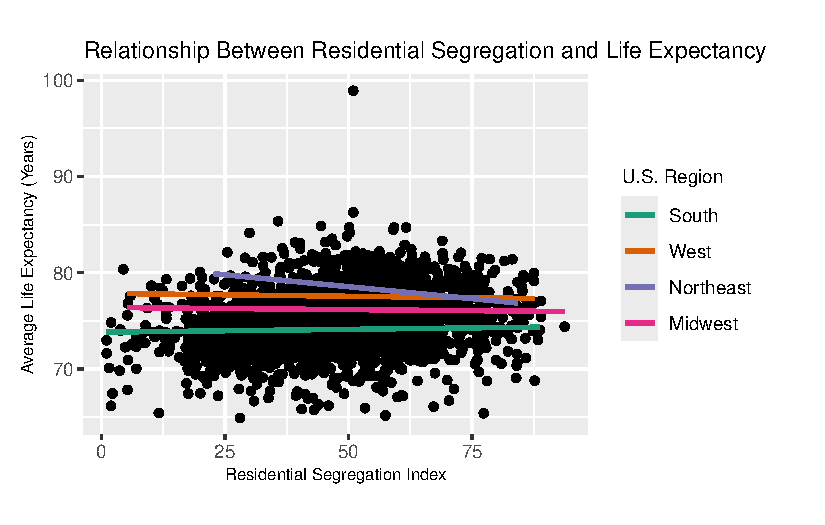
\includegraphics{paper_files/figure-pdf/unnamed-chunk-10-1.pdf}

\newpage

\emph{Table 2: MLR Results For Average Life Expectancy Outcome}

\begin{table}
\centering
\begin{tblr}[         %% tabularray outer open
]                     %% tabularray outer close
{                     %% tabularray inner open
colspec={Q[]Q[]Q[]Q[]Q[]Q[]},
cell{1}{2}={c=5,}{halign=c,},
column{1}={halign=l,},
column{2}={halign=c,},
column{3}={halign=c,},
column{4}={halign=c,},
column{5}={halign=c,},
column{6}={halign=c,},
row{1}={halign=c,},
}                     %% tabularray inner close
\toprule
& (1) &  &  &  &  \\ \cmidrule[lr]{2-6}
& Est. & S.E. & 2.5 \% & 97.5 \% & p \\ \midrule %% TinyTableHeader
(Intercept)                             & \num{65.88}    & \num{0.27}    & \num{65.34}    & \num{66.41}   & \num{<0.01} \\
Residential Segregation Index (RSI)     & \num{0.00715}  & \num{0.00332} & \num{0.00065}  & \num{0.01366} & \num{0.03}  \\
Region-West                             & \num{1.96}     & \num{0.69}    & \num{0.60}     & \num{3.32}    & \num{<0.01} \\
Region-Northeast                        & \num{2.92}     & \num{0.84}    & \num{1.27}     & \num{4.57}    & \num{<0.01} \\
Region-Midwest                          & \num{1.91}     & \num{0.44}    & \num{1.06}     & \num{2.77}    & \num{<0.01} \\
Percentage With Access to Healthy Foods & \num{0.0040}   & \num{0.0062}  & \num{-0.0082}  & \num{0.0162}  & \num{0.52}  \\
Percentage of Uninsured Adults          & \num{0.0328}   & \num{0.0075}  & \num{0.0181}   & \num{0.0476}  & \num{<0.01} \\
Median.Household.Income                 & \num{1.3e-04}  & \num{2.7e-06} & \num{1.2e-04}  & \num{1.3e-04} & \num{<0.01} \\
RSI*Region-West                         & \num{-0.00032} & \num{0.01164} & \num{-0.02313} & \num{0.02250} & \num{0.98}  \\
RSI*Region-Northeast                    & \num{-0.013}   & \num{0.014}   & \num{-0.040}   & \num{0.015}   & \num{0.36}  \\
RSI*Region-Midwest                      & \num{-0.0075}  & \num{0.0075}  & \num{-0.0222}  & \num{0.0072}  & \num{0.32}  \\
\bottomrule
\end{tblr}
\end{table}

\paragraph{Model Assessment}\label{model-assessment}

The adjusted R-squared value for the model was 0.6065, indicating that a
majority of the variability in life expectancy was explained by the
socioeconomic and racial predictors included in the model. In conducting
diagnostics on the multilinear regression model, we first checked to see
if the model met assumptions of linearity, independence, normality, and
homoscedasticity. The residuals vs.~fitted plot showed relatively equal
variance and no discernible pattern, meaning that the linearity and
homoscedasticity assumptions were reasonably met. In addition, because
each observation in the dataset represented a unique county in the U.S.,
independence could be reasonably assumed. Assessing the Q-Q Plot for
normality, the residual distribution was approximately normal, despite a
slight divergence on both tails of the plot. Cook's distance was also
assessed using the residuals vs.~leverage plot; no points were found to
be influential. There was a high leverage point (Mineral County,
Nevada), and refitting the model without this point yielded no
substantial changes in the coefficient estimates for statistically
significant predictors; however, the \emph{p}-value for residential
segregation increased from 0.031 to 0.054. Finally, with a VIF
\textless2 for all predictors, there was little to no multicollinearity
among the predictors.

\subsection{Question 2}\label{question-2}

\paragraph{Model Results}\label{model-results-1}

Table 3 below displays the odds ratio results from the logistic
regression model for school funding adequacy, with the South as the
baseline category for the categorical region variable. While all
estimates are statistically significant at the 0.05 significance level,
exponentiated regression coefficients from the logistic model
demonstrate that a county's median household income and median property
tax have almost no impact on the odds of its schools being adequately
funded. Our results demonstrate that a one unit increase to the
residential segregation index increases the odds of school funding
adequacy by 0.02 times, allowing us to conclude that residential
segregation has a minimal effect on the odds of the school being
adequately funded. Figure 2 demonstrates an interesting trend---each
region shows a different relationship between the residential
segregation distribution of adequately and inadequately funded
schools,~pointing to a potential interaction between region and
segregation. ~

Region has a substantial impact on the odds of school funding
adequacy.~Being located in the Northeast or the Midwest has the greatest
impact on how well a school is funded, with the odds of adequate school
funding being over 200 times higher in a Northeast county compared to a
Southern county, and the odds of adequate school funding being over 3
times higher in a Midwest county compared to a Southern county, holding
all other variables constant. Such disparities across the country are
caused by a number of factors, including: (1) capacity - how well off a
state is based on its economy and resources, and (2) effort - the
state's willingness to provide funding for education. Wealthier states
with a high fiscal capacity, (typically those in the Northeast), have
more funding available to spend on education than states with more
limited resources (typically those in the South and the West).~

In comparing our full model (with predictor variables for residential
segregation, median household income, median property tax, and region)
to a model including all of these variables except for region, we found
that there is statistical significance in the deviance between the
residuals of the full model and reduced. As such, we can conclude that
including region as a predictor refines and creates a better fit for our
model.

\emph{Figure 2: Relationship Between Residential Segregation, Region, \&
School Funding Adequacy}

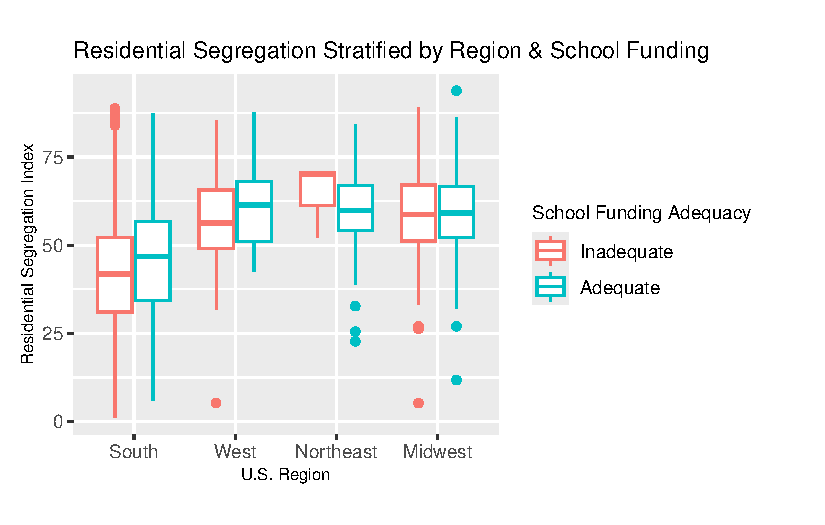
\includegraphics{paper_files/figure-pdf/unnamed-chunk-22-1.pdf}

\emph{Table 3: Logistic Regression Results For School Funding Adequacy
Outcome}

\begin{table}
\centering
\begin{tblr}[         %% tabularray outer open
]                     %% tabularray outer close
{                     %% tabularray inner open
colspec={Q[]Q[]Q[]Q[]Q[]Q[]},
cell{1}{2}={c=5,}{halign=c,},
column{1}={halign=l,},
column{2}={halign=c,},
column{3}={halign=c,},
column{4}={halign=c,},
column{5}={halign=c,},
column{6}={halign=c,},
row{1}={halign=c,},
}                     %% tabularray inner close
\toprule
& (1) &  &  &  &  \\ \cmidrule[lr]{2-6}
& Est. & S.E. & 2.5 \% & 97.5 \% & p \\ \midrule %% TinyTableHeader
(Intercept)                         & \num{0.00135} & \num{0.00050} & \num{0.00064} & \num{0.00273} & \num{<0.01} \\
Residential Segregation Index (RSI) & \num{1.0196}  & \num{0.0041}  & \num{1.0117}  & \num{1.0277}  & \num{<0.01} \\
Median Household Income, USD        & \num{1.0e+00} & \num{5.5e-06} & \num{1.0e+00} & \num{1.0e+00} & \num{<0.01} \\
Median Property Tax, USD            & \num{1.0e+00} & \num{8.5e-05} & \num{1.0e+00} & \num{1.0e+00} & \num{0.01}  \\
Region-West                         & \num{1.83}    & \num{0.35}    & \num{1.26}    & \num{2.66}    & \num{<0.01} \\
Region-Northeast                    & \num{232}     & \num{141}     & \num{82}      & \num{974}     & \num{<0.01} \\
Region-Midwest                      & \num{3.84}    & \num{0.52}    & \num{2.95}    & \num{5.02}    & \num{<0.01} \\
\bottomrule
\end{tblr}
\end{table}

\paragraph{Model Assessment}\label{model-assessment-1}

To assess logistic regression assumptions, we first plotted each
numerical predictor against the log odds of school funding adequacy. All
plots showed a mostly linear relationship, indicating that the linearity
assumption was largely met; interestingly, different linear trends were
observed within each plot based on region, further supporting potential
interaction effects between region and the three numerical predictors.
GVIF for all predictors ranged between 1 and 3, suggesting that there
could be moderate multicollinearity between predictors, but not enough
to warrant a reconsideration of included variables. Cook's distance was
also less than 0.05 for all points, meaning that there were no highly
influential observations in the model. Evaluating our model, we found
that the logistic regression model demonstrated a strong overall
performance with an accuracy rate of 80.33\%. The model had a high
sensitivity of 91\%, indicating that it accurately predicted 91\% of
actual positive cases of adequate school funding when evaluated on our
dataset. However, it had a 60\% specificity rate, highlighting it
correctly identified cases of inadequate school funding only 60\% of the
time. Overall, looking at the ROC curve below, the AUC is 0.858,
indicating a moderately strong discriminate ability.~

\subsection{\texorpdfstring{\textbf{Conclusion}}{Conclusion}}\label{conclusion}

In our analysis, we observed the significant impact of the regional
location of a county on both its average life expectancy (a health
indicator) and school funding adequacy (an educational indicator)--two
key components of societal and individual well-being. Life expectancy is
highest in the Northeast, followed by the Midwest, West, and South,
while school funding adequacy is significantly greater in the Northeast
and Midwest compared to the South. Our findings highlight substantial
differences in both outcomes between regions, which are often caused by
different economic capabilities and different allocations of resources
among countries. This study provides empirical evidence that underscores
the importance for equitable social policies and targeted investments to
address regional disparities and promote well-being across all
communities.

Our analysis faced limitations due to missing data, which restricted the
dataset to 33 states and reduced the generalizability of our findings.
Additionally, some variables were drawn from different years between
2018 and 2022, requiring us to assume that trends remained consistent
over a 1--5 year period and that time was an insignificant factor;
however, this may not actually be the case.

Future studies could look at additional interaction effects with region
and incorporate more social variables to enhance the analysis. For
example, integrating a dataset on employment rates and school
performance could offer deeper insights into how socioeconomic factors
shape life expectancy and educational funding, complementing existing
variables in our models. Another direction for future work is to delve
deeper into understanding the surprising findings regarding the effects
of uninsured adult percentage and residential segregation on life
expectancy. Expanding the dataset to include a temporal scope, and
finding more complete sources of data on variables of interest so that
no states have to be excluded from the analysis, would also contribute
to a more comprehensive understanding.

\subsection{\texorpdfstring{\textbf{Appendix}}{Appendix}}\label{appendix}

\emph{Table A1: Summary Statistics For All Variables}

\subsection{\texorpdfstring{\protect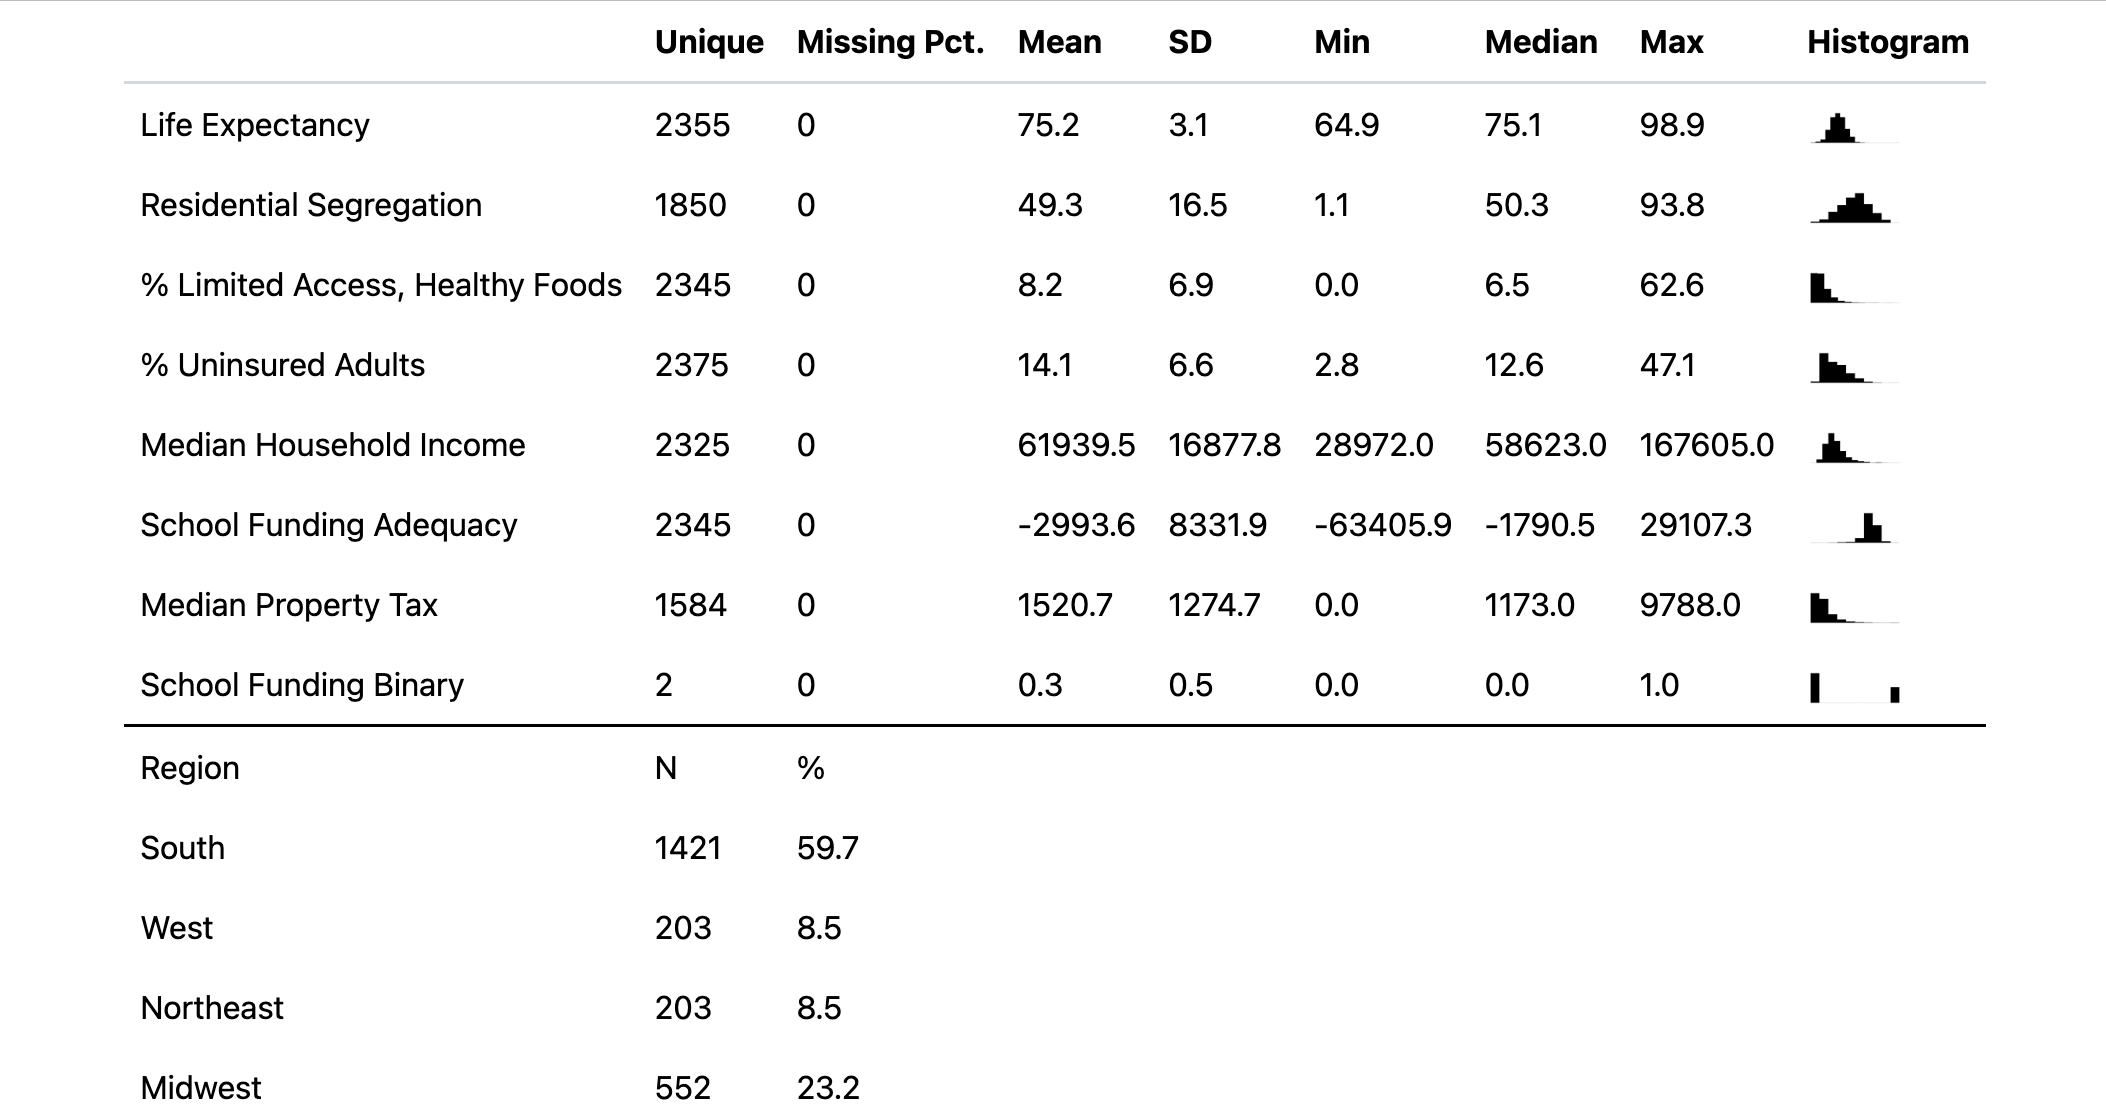
\includegraphics{images/clipboard-2912764107.png}}{}}\label{section}

\subsection{\texorpdfstring{\textbf{References}}{References}}\label{references}

\begin{enumerate}
\def\labelenumi{\arabic{enumi}.}
\item
  National Academies of Sciences, Engineering, and Medicine. (2017).
  \emph{Communities in action: Pathways to health equity.} Washington,
  DC: The National Academies Press. Retrieved from
  \url{https://www.ncbi.nlm.nih.gov/books/NBK425845/}
\item
  Stanford Center for Opportunity Policy in Education. (2013.). How to
  close the opportunity gap: Key policy recommendations. Retrieved from
  \url{https://edpolicy.stanford.edu/sites/default/files/Opp\%20Gap\%20Policy\%20Recommendations.pdf}
\item
  County Health Rankings \& Roadmaps. (n.d.). \emph{About us.} Retrieved
  December 8, 2024, from
  \url{https://www.countyhealthrankings.org/about-us}
\item
  Steven Ruggles, Sarah Flood, Matthew Sobek, Daniel Backman, Annie
  Chen, Grace Cooper, Stephanie Richards, Renae Rodgers, and Megan
  Schouweiler. IPUMS USA: Version 15.0 {[}dataset{]}. Minneapolis, MN:
  IPUMS, 2024. Retrieved from \url{https://doi.org/10.18128/D010.V15.0}
\item
  Halpert, C. (2014). Census regions {[}GitHub repository{]}. GitHub.
  \url{https://github.com/cphalpert/census-regions}
\item
  USDA. (2022). \emph{Documentation}. Economic Research Service.
  https://www.ers.usda.gov/data-products/food-access-research-atlas/documentation/
\item
  County Health Rankings \& Roadmaps. (2024). \emph{Residential
  segregation - Black/White.} University of Wisconsin Population Health
  Institute. Retrieved from
  \url{https://www.countyhealthrankings.org/health-data/health-factors/social-economic-factors/family-and-social-support/residential-segregation-blackwhite?utm_source=chatgpt.com&year=2024}
\item
  Chetty, R., Stepner, M., Abraham, S., Lin, S., Scuderi, B., Turner,
  N., Bergeron, A., \& Cutler, D. (2016). The Association Between Income
  and Life Expectancy in the United States, 2001-2014. \emph{JAMA},
  \emph{315}(16), 1750--1766. https://doi.org/10.1001/jama.2016.4226
\item
  County Health Rankings \& Roadmaps. (2024). \emph{School funding
  adequacy.} University of Wisconsin Population Health Institute.
  Retrieved from
  \url{https://www.countyhealthrankings.org/health-data/health-factors/social-economic-factors/education/school-funding-adequacy?utm_source=chatgpt.com&year=2024}
\end{enumerate}



\end{document}
